
\section{High Performance Parallel Computing}\label{sec:hppc}

Now that we have taken a look at the computations performed by the xTB method, we can begin to see that the steps are the same for all molecules, and that the exact amount of steps are identical between isomers. Isomers are molecules that are identical in their composition of atoms, that is, they have the same molecular formula, and differ only in the relative positions between atoms or the bonds between them.
This project focuses on large isomer spaces of fullerenes in the range \(C_{20}, \cdots, C_{200} \) which is a total of $2157751423$ molecules, or in other words in the order of $10^9$. A fullerene is a molecule consisting only of carbon atoms where each atom has three neighbors and is arranged such that the molecule produces a mesh of exactly $12$ pentagonal faces and the rest being hexagonal faces.

\begin{figure}[H]
\centering
\begin{tikzpicture}[carbon/.style={circle, draw=black, fill=white, minimum size=12pt, inner sep=2pt}]

  % Central carbon atom
  \node[carbon] (C0) at (0,0) {C};

  % Neighboring carbon atoms at 120° intervals
  \foreach \angle/\name in {90/C1, 210/C2, 330/C3} {
    \node[carbon] (\name) at ({2*cos(\angle)}, {2*sin(\angle)}) {C};
    \draw (C0) -- (\name);
  }

  \path (C1) -- ++(.7,.7)
    node[pos=0.5, sloped] {$\hdots$};
  \path (C1) -- ++(-.7,.7)
    node[pos=0.5, sloped] {$\hdots$};

  \path (C2) -- ++(0,-.9)
    node[pos=0.5, sloped] {$\hdots$};
  \path (C2) -- ++(-.9,0)
    node[pos=0.5, sloped] {$\hdots$};

  \path (C3) -- ++(0,-.9)
    node[pos=0.5, sloped] {$\hdots$};
  \path (C3) -- ++(.9,0)
    node[pos=0.5, sloped] {$\hdots$};
\end{tikzpicture}
\caption{Each carbon atom in a fullerene has exactly 3 neighboring carbon atoms.}
\label{fig:carbon-degree}
\end{figure}

For each isomerspace we essentially have two matrices, one for the coordinates of each carbon atom, and one containing the three neighbors for each of the atoms. The first matrix as seen in \autoref{fig:isomerspace_atom_coords}, is of size $N \times 3 \times M$ where $N$ is the amount of atoms for each of the fullerenes within the same isomerspace, $3$ is the three coordinates for each atom, and $M$ is the amount of fullerenes within the isomerspace. The second matrix as seen in \autoref{fig:isomerspace_atom_neighbors}, is the exact same, but instead of coordinates it holds the indices for the three neighboring carbon atoms. The xTB method only needs the positions for each atom, so we are not concerned with the second matrix.

% TODO: Is it true that we do not need the second matrix?

\begin{figure}[H]
\centering
\begin{minipage}{.45\textwidth}
  \centering
  \begin{tikzpicture}
  \def\xs{1} %shift in x direction
  \def\ys{0.5} %shift in y direction
  \def\nm{5} % number of 2d matrices in the 3d matrix
  \foreach \x in {1,2,...,\nm}
  {

  \matrix [draw, % for the rectangle border
           fill=white, % so that it is not transparent
           ampersand replacement=\&,
           row sep=0pt
          ] %see explanation
  (mm\x)%give the matrix a name
  at(-\x * \xs, -\x * \ys) %shift the matrix
  {
          \node {$x$ $y$ $z$};\\
          \node {$x$ $y$ $z$};\\
          \node {$x$ $y$ $z$};\\
          \node {   $\vdots$   };\\
  };
  }



  \draw [dashed,gray](mm1.north west) -- (mm\nm.north west);
  \draw [dashed,gray](mm1.north east) -- (mm\nm.north east);
  \draw [dashed,gray](mm1.south east) -- (mm\nm.south east);

  % Vertical label (Height)
  \node at ([xshift=-4mm]$(mm\nm.south west)!0.5!(mm\nm.north west)$) {$N$};

  % Horizontal label (Width)
  \node at ([yshift=-4mm]$(mm\nm.south west)!0.5!(mm\nm.south east)$) {$3$};

  % Depth label
  \path (mm1.south east) -- (mm\nm.south east)
      node[pos=0.5, sloped, below=4pt] {$M$};

  % sloped hdots behind first matrix on the right side
  \path (mm1.east) -- ++(\xs/2,\ys/2)
      node[pos=0.5, sloped] {$\hdots$};

  \end{tikzpicture}
  \caption{Matrix with the atom coordinates for each fullerene within an isomerspace. The 3-dimensional matrix holds the $3$ coordinates for each of the $N$ carbon atoms for all $M$ fullerenes in a given isomerspace.}
  \label{fig:isomerspace_atom_coords}
\end{minipage}%
\hspace{.05\textwidth}
\begin{minipage}{.45\textwidth}
  \centering
  \begin{tikzpicture}
  \def\xs{1.2} %shift in x direction
  \def\ys{0.5} %shift in y direction
  \def\nm{5} % number of 2d matrices in the 3d matrix
  \foreach \x in {1,2,...,\nm}
  {

  \matrix [draw, % for the rectangle border
           fill=white, % so that it is not transparent
           ampersand replacement=\&,
           row sep=0pt
          ] %see explanation
  (mm\x)%give the matrix a name
  at(-\x * \xs, -\x * \ys) %shift the matrix
  {
          \node {$a_1$ $a_2$ $a_3$};\\
          \node {$a_1$ $a_2$ $a_3$};\\
          \node {$a_1$ $a_2$ $a_3$};\\
          \node {   $\vdots$   };\\
  };
  }



  \draw [dashed,gray](mm1.north west) -- (mm\nm.north west);
  \draw [dashed,gray](mm1.north east) -- (mm\nm.north east);
  \draw [dashed,gray](mm1.south east) -- (mm\nm.south east);

  % Vertical label (Height)
  \node at ([xshift=-4mm]$(mm\nm.south west)!0.5!(mm\nm.north west)$) {$N$};

  % Horizontal label (Width)
  \node at ([yshift=-4mm]$(mm\nm.south west)!0.5!(mm\nm.south east)$) {$3$};

  % Depth label
  \path (mm1.south east) -- (mm\nm.south east)
      node[pos=0.5, sloped, below=4pt] {$M$};

  % sloped hdots behind first matrix on the right side
  \path (mm1.east) -- ++(\xs/2,\ys/2)
      node[pos=0.5, sloped] {$\hdots$};

  \end{tikzpicture}
  \caption{Matrix holding an adjacency list of $3$ neighbors for each carbon atom for all fullerenes in a given isomerspace.}
  \label{fig:isomerspace_atom_neighbors}
\end{minipage}
\end{figure}


The xtb program takes a single molecule as input, but the fact that fullerenes in the same isomerspace executes the same series of instructions, makes a great case for lockstep parallelism. Running computations in lockstep means doing the exact same instructions in parallel, and if we can do this, then we can efficiently utilize the single instruction, multiple threads (SIMT) execution model. The SIMT model is used when a warp scheduler dispatches a single instruction to all threads within a warp. All of the threads in the warp will then execute the instruction simultaniously, which means that they are synchronized at a hardware level. This perfect as it means that we can use warps to execute instructions for multiple fullerenes in lockstep. With this in mind, instead of feeding the program a single fullerene at a time, we want to give it a complete isomerspace so that we can utilize all threads on one or even multiple GPUs. The largest isomerspace we consider is $C_{200}$, which is $214127742$ fullerenes, or in other words in the order of $10^8$.

It takes around $30$ seconds for a 12th generation Intel mobile processor to run xtb on a single $C_{200}$ fullerene. Going through the whole isomerspace on this CPU would take about $204$ years to complete. This is a bit long to wait for a failed run, and by that time we will probably have achieved more efficient ways of computation, or the world might simply have more pressing matters than keeping this computer alive. The degree of lockstep parallelism scales with the isomerspace, and since there are no interdependencies between the molecules, this makes it a perfect case for horizontal scaling by using hundreds or even thousands or GPUs. The CPU used has $12$ cores and $24$ threads, $12$ of which can run in parallel. An NVIDIA GPU has hundredthousands of threads and tenthousands of CUDA cores, though these cores are not equivalent to CPU cores, and we can in general not compare the relative performance between the two by looking at this. Something that is typically compared though, is the theoretical throughput of floating point operations per second (FLOPS). The top of the line AMD EPYC 9965 CPU has a theoritical throughput of $27.648$ TeraFLOPS (TFLOPS) for $32$-bit floating point values\cite{amd-epyc-performance}, while the NVIDIA A100 has $156$ TFLOPS\cite{nvidia-a100-architecture}. From these observations we can say that the GPU is much more capable of massive parallelism, which is what we seek for these massive isomerspaces.
%as they refer to the amount of arithmetic logic units (ALUs), while a modern CPU core has multiple ALUs.

%Distributing the isomerspace over $1000$ threads would cut this down to a measly $2.5$ months. This is still a lot and it also assumes that the clock cycles on a GPU is just as fast as on the Intel CPU, which they are not, but this is fine, because we have a lot more than $1000$ threads to work with.

%A single C200 molecule takes ... so this many would take... distributing it over 1000 would take this much wall time..
%By using multiple GPUs we can distribute these huge isomerspaces 

%We want to run molecules in lockstep. Fullerenes in the same isomerspace does the same steps. We have to find the upperbound for iterations and array allocations to run the exact same instructions for each. If we do the exact same on molecules within the same warp, then we can get a constant flow of throughput since we will need no barriers. In this case, synchronization is not needed within the same warp, so no barriers! Doing the exact same on the level of isomers is great, because we have so many, so we can keep scaling up the hardware to use 100, 1000 GPUs and we will still be able to utilize all cores because the isomerspace sizes scale in the order of magnitude of 10\^9 or something.

\subsection{Case Study}

To get an idea of the scale of parallelism we can achieve on a single GPU, we will take a look at the memory specifications of the NVIDIA A100 GPU. We hope to use this to get an idea of how many fullerenes can fit into memory.

Using all the levels of memory on a GPU efficiently is crucial to achieve high performance in parallel computing tasks. Let us therefore take a moment to familiarize ourselves with the different types typically found in the memory hiearchy on a GPU. Below you will find an overview of the main memory levels with short explanations for each of them:

\begin{itemize}
  \item Global - Accessible from all threads on the GPU. This is the largest but also the slowest pool of memory in terms of latency.
  \item Shared - Tied to a thread block (or workgroup), so it can be accessed by the threads in the same block. This pool of memory is smaller but faster to access than global memory.
  \item Register Memory - Each thread on a GPU has private access to a number of registers. This is the fastest type of memory used to store local variables and intermediate results.
  %\item Local Memory - Also private to each thread. This type is slower than register memory and is usually used when there is insufficient space for variables on the registers of a thread.
\end{itemize}

% There are 4 warp schedulers(1 per SMSP) so 4 per SM. These schedule up to 16 warps concurrently where each is either from one or several block, from one or several kernels. 4 * 16 = 64 max warps.
% 4 schedulers * 32 threads/warp = 128 threads/cycle
% Each scheduler can schedule up to 2 instructions per cycle? so 256 instructions/cycle
% This is for Kepler, check for Ada
%https://forums.developer.nvidia.com/t/how-to-the-a100-gpu-s-maximum-warps-per-scheduler/300096
% Table 5
%https://images.nvidia.com/aem-dam/en-zz/Solutions/data-center/nvidia-ampere-architecture-whitepaper.pdf

% Good SM explanation
% https://modal.com/gpu-glossary/device-hardware/streaming-multiprocessor

% 64000 is wrong! 64K, the K means 2^10, so it is 65536.
% This matches the nvidia whitepaper above where it states the whole number as 65536 32-bit registers / SM.

% Smid regnestykker ind i en klar "example" for Ada, og skriv hvad de skal bruges til!

We will specifically look at the NVIDIA A100 GPU \cite{nvidia-a100-architecture}, which has $40$ GB of memory and $108$ SMs each with $64$ FP32 CUDA cores and $4$ tensor cores resulting in a total of $6912$ CUDA cores and $432$ tensor cores.

To find out how many fullerenes worth of coordinate data can fit into global memory, we can use the following equation:

\begin{figure}[H]
\begin{equation}
\begin{split}
        GlobalMemFullereneCapacity &= \floor*{\frac{GlobalMemInBits}{FullereneAtomCount \times 3 \times 32}}
\end{split}
\end{equation}
\caption{The amount of 3-dimensional fullerene coordinate data that fits in global memory. The $3 \times 32$ comes from the three $32$-bit floating point numbers that represents the 3-dimensional coordinates. This equation does not consider other data such as results or intermediate values.}
\end{figure}

\begin{figure}[H]
\begin{equation}
\begin{split}
        MinimumBatchesToFitIsomerspace &= \ceil*{\frac{IsomerspaceSize}{GlobalMemFullereneCapacity}}
\end{split}
\end{equation}
\caption{The minimum number of batches required to process a complete isomerspace in global memory.}
\end{figure}

Be aware that this equation does not consider any space needed for the results or any intermediate values, but we can use this equation to calculate the minimum amount of batches needed to process the whole isomerspace. If we want to process the whole isomerspace at once, then we might need to add additional GPUs. For example, the $C_{200}$ isomerspace needs a minimum of $13$ GPUs with $40$ GB of global memory each.

We are also interested in knowing how much non-global memory is available to each xTB computation. Knowing this will tell us how many of the threads, warps, and blocks we can utilize on the GPU. To figure this out, we first need to know how much of the various memory levels are available to a single thread if distributed over all threads.

Each SM has up to $164$ KB of shared memory and is divided into four partitions, each containing a $64$ KB register file, an one warp scheduler, $16$ CUDA Cores dedicated for processing FP32 operations, $16$ CUDA Cores for processing INT32 operations, $8$ CUDA Cores for processing FP64 operations, and a tensor core, which is specialized for matrix operations. See \autoref{fig:a100-SM-architecture} for a figure of the SM architecture.

\begin{figure}[H]
\centering
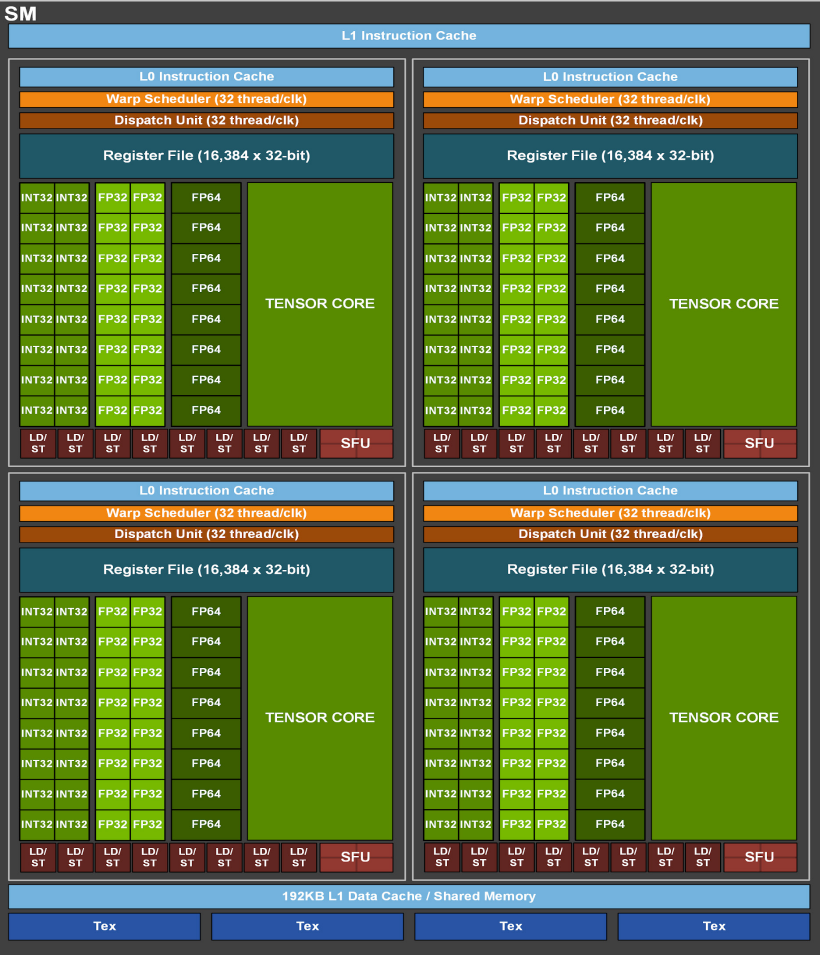
\includegraphics[scale=0.3]{images/nvidia-a100-architecture}
\caption{The NVIDIA A100 Architecture for a streaming-multiprocessor. \cite[Figure 5]{nvidia-a100-architecture}}
\label{fig:a100-SM-architecture}
\end{figure}

There are a maximum of $64$ warps per SM, so each warp scheduler has $16$ warps allocated to them. Each warp has $32$ threads, so if we distribute a register file over the $512$ threads for an SM, then each of them have $320$ bytes (see \autoref{eq:reg_per_thread}). If we need to allocate more memory per thread, then we can utilize fewer of the threads.

To get the amount of shared memory available to each thread when distributed evenly, we can use \autoref{eq:shared_per_thread}. There is $164$ KB of shared memory per SM, so each thread has $80$ bytes to work with.

\begin{equation}
\begin{split}
        RegisterMemoryPerThread &= \frac{RegisterFile}{WarpsPerPartition \times ThreadsPerWarp} \label{eq:reg_per_thread}
\end{split}
\end{equation}

\begin{equation}
\begin{split}
        SharedMemoryPerThread &= \frac{SharedMemoryPerSM}{WarpsPerSM \times ThreadsPerWarp} \label{eq:shared_per_thread}
\end{split}
\end{equation}


Depending on the upperbound on intermediate data required by the GFN2-xTB algorithm, we can tweak the amount of non-global memory available to each fullerene by using fewer threads, warp, and blocks. For example, using only $16$ of the $32$ threads in each warp will double the available register and shared memory for each thread. There is a point of diminishing returns as a single thread is limited to a maximum of $255$ $32$-bit registers. In the case that the non-global memory alone is not enough to hold the intermediate data of a molecule, then we will need to also utilize global memory. Shared memory has a latency of $20$ to $30$ cycles while global memory has a latency of $200$ to $1000$ cycles \cite{nasa-nvidia-basics}. Global memory is slow to access, so when used it becomes especially important to place data strategically to allow for coalesced access.

%Each SM has a maximum of $24$ blocks and a maximum of $48$ warps. This adds up such that full utilization can be achieved when each block has $2$ warps allocated. A warp has $32$ threads, so an SM has a total of $1536$ threads when each of its $24$ blocks has two warps.
%%By using \autoref{eq:reg_mem_utilized_per_sm} we can see that this configuration utilizes $251.9$ KB of the register memory available to each of the SMs.
%
%\begin{equation}
%\begin{split}
%  WarpsPerBlock &= \floor*{\frac{WarpsPerSM}{BlocksPerSM}}
%\end{split}
%\end{equation}
%
%\begin{equation}
%\begin{split}
%  ThreadsPerBlock &= WarpsPerBlock \times ThreadsPerWarp
%\end{split}
%\end{equation}
%
%\begin{equation}
%\begin{split}
%  RegistersPerThread &= \floor*{\frac{RegistersPerSM}{BlocksPerSM \times ThreadsPerBlock}}
%\end{split}
%\end{equation}
%
%\begin{equation} \label{eq:reg_mem_utilized_per_sm}
%\begin{split}
%  RegisterMemoryUtilizedPerSM =\\
%  &BlocksPerSM\\
%  &\times ThreadsPerBlock\\
%  &\times RegistersPerThread\\
%  &\times BitsPerRegister
%\end{split}
%\end{equation}
%
%BlocksPerSM and BitsPerRegister are constants found in the specification for the GPU architecture.
%
%With this, each block in an SM has $10.496$ KB of register memory to work with, and thus each thread has $164$ bytes.
%
%\begin{equation}
%\begin{split}
%  \frac{251.904}{24} &= 10.496 \text{ KB}
%\end{split}
%\end{equation}
%
%\begin{equation}
%\begin{split}
%  \frac{251904}{1536} &= 164 \text{ bytes}
%\end{split}
%\end{equation}
%
%The shared memory capacity per SM is $100$ KB and a single block can have a maximum of $99$ KB. This gives each block about $4.16$ KB of shared memory, meaning that the $64$ threads in a block will have $65$ bytes each.
%
%\begin{equation}
%\begin{split}
%  \frac{100}{24} &= 4.166 \text{ KB}
%\end{split}
%\end{equation}
%
%\begin{equation}
%\begin{split}
%  \frac{4166}{64} &= 65.09 \text{ bytes}
%\end{split}
%\end{equation}
%
%The Ada Lovelace architecture has a total of $128$ SMs and it also has a $98304$ KB L2 cache. This results in a total of $3072$ blocks that each has $32$ KB of the L2 Cache. All of this combined gives each block a total of $46.656$ KB of non-global memory.
%
%\begin{equation}
%\begin{split}
%  10.496 \text{ KB} + 4.166 \text{ KB} + 32 \text{ KB} &= 46.662 \text{ KB}
%\end{split}
%\end{equation}
%
%Distributing the global memory across the blocks gives each of them $26.042$ MB. Combined with the non-global memory, this results in each block having a total of $26.088$ MB of memory.

%\subsection{Optimizing GPU Configuration for Isolated Molecules}
%
%Computing xTB-GFN2 for a molecule is completely isolated, so if we do the whole xTB computation in lockstep, then we only have to concern ourselves with how many warps and blocks a single molecule needs in order to keep all its data in device memory. When we know these details, then we can simply scale up the number of molecules to be computed in lockstep until all the resources on the GPU are saturated. With this approach, expanding to multiple GPUs should be rather trivial as there are no interdependencies.
%
%The exact space needed to compute the GFN2 method of xTB for a single fullerene is not yet clear to us, and it will also vary based on the size of the fullerene. To make finding the most optimal GPU configuration easier when optimizing for most possible parallel xTB computations, we have developed a script that computes such a configuration based on the space requirement of a single molecule.
%
%\begin{figure}[h!]
%\begin{minted}{python}
%  def compute(bytes_per_molecule):
%    mb_per_molecule = bytes_per_molecule / 1_000_000
%
%    threads_per_molecule = compute_threads_per_molecule(mb_per_molecule)
%    warps_per_molecule = compute_warps_per_molecule(threads_per_molecule)
%    molecules_per_block = compute_molecules_per_block(warps_per_molecule)
%
%    print_utilization(warps_per_molecule, molecules_per_block)
%
%    print(f"MB per molecule: {mb_per_molecule} MB")
%    print(f"Threads per molecule: {threads_per_molecule}")
%    print(f"Warps per molecule: {warps_per_molecule}")
%    print(f"Molecules per block: {molecules_per_block}")
%\end{minted}
%  \caption{This is the top-level function for computing the optimal number of warps needed per molecule when optimizing for most possible parallel xTB computations on a single GPU specifically for the Ada Lovelace architecture.}
%\end{figure}
%
%The output of the script has information on how many threads are required for a single molecule, how many warps this fits within. It also includes general information about the utilization of the GPUs resources with the configuration presented. An example of the full output can be seen in \autoref{fig:gpu-mem-output}.
%
%
%\begin{figure}[h!]
%\begin{minted}[linenos=false]{text}
%| Global memory | L2 cache | Total SMs | Threads per warp |
%|    80.0 GB    | 98304 KB |    128    |        32        |
%| Threads Available | Threads Used | Blocks Available | Blocks Used |
%|      196608       |    196608    |       3072       |    3072.0   |
%
%#################################### Per SM ####################################
%| Warps | Blocks | Registers | Shared Memory | Threads Available | Threads Used |
%|  48   |   24   |   64000   |    100 KB     |       1536        |     1536     |
%| Blocks Available | Blocks Used |
%|        24        |     24.0    |
%
%########################### Per Block ###########################
%| L2 Cache | Register Mem | Shared Mem | Global Mem | Total mem |
%| 32.0 KB  |  10.496 KB   |  4.167 KB  |  26.042 MB | 26.088 MB |
%
%MB per molecule: 8.3 MB
%Threads per molecule: 18
%Warps per molecule: 1
%Molecules per block: 2
%\end{minted}
%\caption{This is the output of our script for computing an optimal GPU configuration when a single molecule needs $8.3$ MB of memory.}
%\label{fig:gpu-mem-output}
%\end{figure}
%
%In \autoref{fig:gpu-mem-output} each molecule is $8.3$ MB and thus requires the memory of $18$ threads. Each warp has $32$ threads, so in this case a single molecule fits within a single warp. With $24$ blocks and $48$ warps per SM, all blocks can have $2$ warps each, which in this scenario means that $2$ molecules can be computed in parallel within a single block. This space requirement for a molecule is just an example and in no way guaranteed to be representative of the actual requirements of fullerenes of any size.
%
%
%%The electrostatic energy term depends on the initial Huckel energy term H0, P, dq, dqsh, atomicGam, shellGam, jmat\_flat, shift...
%%
%%Instead of giving a bad approximation then just explain the equations and how to use the script.
%%
%%83GB for 10000 C200
%%8.3 MB for each molecule
%%SMs has max 48 warps
%%each warp has 32 threads
%%64000 32bit registers per SM
%%each thread can max use 255 registers
%%max thread blocks per SM is 24
%%two thread blocks to make use of all 48 warps
%%shared memory capacity per SM 100KB
%%maximum shared memory per thread block is 99KB
%%SMs schedule warps/workgroups/thread blocks
%%we can do ~1536 molecules per SM with this amount of data
%
%
%
%
%%Doing more fine grained parallelization can make use of SIMT(Single instruction multiple threads) like reduction.
%
%
%We cannot do all fullerenes at once for the largest isomerspaces, so they have to be computed in batches. To achieve good speedups we also have to utilize the GPU efficiently.

\subsection{Data Coalescing}

% TODO: Udvid og strukturer klart. Forklar at det eksisterende xTB program tager et molekyle ad gangen, og hvad vi får ud af at arbejde på flere samtidigt, that is, at vi nu har muligheden for lockstep parallelisering og at flytte flere molekyler i memory samtidigt.

Our goal is an xTB implementation capable of working with data for several molecules in parallel. This opens the opportunity for coalesced data access if we can structure the data in a way that achieves spacial locality. Spacial locality is achieved when related data is close together in memory such that it can be accessed as a contiguous block. This minimizes cache misses by eliminating random access across cache lines. One way to achieve spacial locality is to store data as structures of arrays (SOA) instead of arrays of structures (AOS) (see \autoref{fig:coalescing}). In order to allow coalesced access to data in device memory, we can essentially realign the data to match the access patterns of our kernels.%Doing this should also decrease the amount of copies needed between host and device memory, resulting in overall faster execution.

\begin{figure}[h]
\centering
\begin{tikzpicture}[
squarednode/.style={
    rectangle,
    draw=black,
    fill=violet,
    text=white,
    thin,
    minimum size=5mm,
    inner sep=0pt, % No inner spacing
    outer sep=0pt, % No outer spacing
},
]

\node[squarednode] (A1) at (0,0) {$A_1$};
\node[squarednode, anchor=west] (A2) at (A1.east)   {$A_2$};
\node[squarednode, anchor=west] (A3) at (A2.east)   {$A_3$};
\node[squarednode, anchor=west] (A4) at (A3.east)   {$A_4$};

\node[squarednode, anchor=west, fill=cyan, text=black] (A1-2) at (A4.east)   {$A_1$};
\node[squarednode, anchor=west, fill=cyan, text=black] (A2-2) at (A1-2.east)   {$A_2$};
\node[squarednode, anchor=west, fill=cyan, text=black] (A3-2) at (A2-2.east)   {$A_3$};
\node[squarednode, anchor=west, fill=cyan, text=black] (A4-2) at (A3-2.east)   {$A_4$};

\node[squarednode, anchor=west, fill=yellow, text=black] (A1-3) at (A4-2.east)   {$A_1$};
\node[squarednode, anchor=west, fill=yellow, text=black] (A2-3) at (A1-3.east)   {$A_2$};
\node[squarednode, anchor=west, fill=yellow, text=black] (A3-3) at (A2-3.east)   {$A_3$};
\node[squarednode, anchor=west, fill=yellow, text=black] (A4-3) at (A3-3.east)   {$A_4$};



\node[squarednode, anchor=west] (A1-4) [below=of A1] {$A_1$};
\node[squarednode, anchor=west, fill=cyan, text=black] (A1-5) at (A1-4.east)   {$A_1$};
\node[squarednode, anchor=west, fill=yellow, text=black] (A1-6) at (A1-5.east)   {$A_1$};

\node[squarednode, anchor=west] (A2-4) at (A1-6.east)   {$A_2$};
\node[squarednode, anchor=west, fill=cyan, text=black] (A2-5) at (A2-4.east) {$A_2$};
\node[squarednode, anchor=west, fill=yellow, text=black] (A2-6) at (A2-5.east)   {$A_2$};

\node[squarednode, anchor=west] (A3-4) at (A2-6.east)   {$A_3$};
\node[squarednode, anchor=west, fill=cyan, text=black] (A3-5) at (A3-4.east)   {$A_3$};
\node[squarednode, anchor=west, fill=yellow, text=black] (A3-6) at (A3-5.east) {$A_3$};

\node[squarednode, anchor=west] (A4-4) at (A3-6.east)   {$A_4$};
\node[squarednode, anchor=west, fill=cyan, text=black] (A4-5) at (A4-4.east)   {$A_4$};
\node[squarednode, anchor=west, fill=yellow, text=black] (A4-6) at (A4-5.east)   {$A_4$};

\draw[->, thick] ($(A2-2.south) + (0.25,-0.25)$) -- ($(A2-6.north) + (0.25,0.25)$);

\node[draw=red, very thick, fit=(A1-4)(A1-5)(A1-6), inner sep=2pt] {};
\node[draw=red, very thick, fit=(A1)(A2)(A3), inner sep=2pt] {};

\end{tikzpicture}
\caption{Transforms arrays of structures where the memory for each structure is laid out contiguously, into a flattened structure of arrays where data relevant for a computation is close together. This way of grouping related data close together achieves spatial locality and allows for coalesced access of the data.}
\label{fig:coalescing}
\end{figure}

This project is part of a larger pipeline, so the fullerene data that is fed to the GFN2-xTB algorithm is already in device memory when we get it. The GFN2-xTB implementation therefore never moves any data between the host and device. As such, data coalescing is something we consider when data is moved from higher to lower levels of memory on a device.

In contrast to a task-parallel model where different instructions are executed in parallel, the threads in a warp is optimized around the single instruction multiple threads model (SIMT). This means that all $32$ threads in a warp can execute the exact same instructions in lockstep, thus being synchronized on a hardware level. To run in lockstep, data access has to complete for all the threads before the warp can advance, so to best utilize the SIMT model we need to fetch the data efficiently in a coalesced manner to minimize latency and maximize throughput.
%To give an example, if a kernel only needs a subset of the fullerene for the current computation, then we should take the same subset for all fullerenes in the isomerspace and place them close together in memory.%Doing this allow us  from a single fetch, than if we also had to fetch the rest of the molecule data between these subsets.

No matter how efficiently we store our data, the throughput will still be bottlenecked by the memory bandwidth if our cores are constantly waiting for new data. To maximize throughput each core has to execute multiple instructions per byte of data. This will ensure that new data can arrive in time for when the cores need it. We will now show how to calculate the required amount of instructions per byte with the A100 GPU as an example. To keep things simple, we will assume that each CUDA core can execute one instruction per clock cycle, and we will only consider the FP32 Cores.

The A100 uses HBM2 DRAM memory, which is organized as five active HBM2 stacks with eight memory dies per stack. Each channel is $128$ bits wide, so a whole die is $1024$ bits wide, which makes a stack $5120$ bits wide. The memory has a double data rate (DDR) of $1215$ MHz. DDR gives us two transfers per clock cycle, so it is effectively $2430$ MHz, or $2.43$ GT/s.

\begin{equation}
\begin{split}
        StackMemoryInBytes &= \frac{ChannelWidth \times ChannelsPerDie \times DiesPerStack}{8}\\
\end{split}
\end{equation}

\begin{equation}
\begin{split}
        MemoryBandwidth &= StackMemoryInBytes \times DataRateInMHz \times GigaTransfersPerSecond\label{eq:memorybandwidth}\\
\end{split}
\end{equation}

Using \autoref{eq:memorybandwidth} with the specifications of the A100 GPU, we get a total memory bandwidth of $1555$ GB/s, which matches the A100 whitepaper from NVIDIA\cite{nvidia-a100-architecture}.

With this bandwidth we can fetch $1555$ bytes per 1GHz clock cycle, so if we use the $6912$ FP32 CUDA Cores on the A100, then each core should execute $5$ instructions per byte fetched.

\begin{equation}
\begin{split}
        InstructionsPerByte &= \ceil*{\frac{CoreCount}{ByteTransfersPer1GHz}}\\
\end{split}
\end{equation}

We did not consider that a single core can execute more than one instruction per cycle, but if we look at the peak FP32 rate of $19.5$ TFLOPS, then we can calculate that we actually need $13$ instructions per byte to reach maximum throughput (see \autoref{eq:instructions-per-byte-given-tflops}).

\begin{equation}
\begin{split}
        InstructionsPerByteGivenTFLOPS &= \ceil*{\frac{TFLOPSInBytes}{ByteTransfersPer1GHz}}\label{eq:instructions-per-byte-given-tflops}\\
\end{split}
\end{equation}


%A complete molecule will most likely not fit in the lower memory levels, so we need to interweave the data in higher levels such that the necessary parts can be accessed as fast as possible. The bottom line is, that when we compute the energies for multiple molecules in the same warp, then we would like to move the necessary data for the molecules at the same time to minimize data accesses to higher levels of memory.


\subsection{Introduction to a Parallel Lockstep Algorithm}

We want to ensure that all threads within a warp can work on different fullerenes in parallel. To achieve this we need to remove branching in the code and place upper bounds on all loops to make sure the exact same work is performed by the threads. Luckily, since we are only working with one type of atom, we can simply replace branches with the case that applies for carbon.

Normally we would have to set upper bounds on all loops to ensure instructions are executed the same amount of times for all atoms. This is not necessary in our case since we only have carbon atoms, because all of them have the same amount of shells, orbitals, electrons and so on.

\subsection{Orbitals as a constant}

This following helper function would never be called in the actual implementation, but instead be computed on the fly. This section will show however, that we never need to compute this at all with fullerenes and can instead store it as a compact constant array. 

\begin{figure}[H]
\begin{minted}{python}
def get_orbitals(atoms: list[int]) -> list[tuple[int]]:
    orbitals = []
    for atom_idx,atom in enumerate(atoms):
        for subshell in range(number_of_subshells[atom]):
            l = angular_momentum_of_subshell[atom][subshell] 
            for orbital in range(l*2+1):
                orbitals.append((atom_idx,atom,subshell,orbital))
    return orbitals
\end{minted}
\caption{The original helper function for computing the orbitals for each atom in a molecule.}
\end{figure}

The orbitals for each atom will always be the same since we are only working with carbon atoms, so we can simply compute the orbitals for the first atom and then use the count of atoms as a bound for how many times we can read the array. This means that we only return an array with the orbitals for the two subshells in the first carbon atom, and we can thus remove the outermost loop.

\begin{figure}[H]
\begin{minted}{python}
def get_orbitals() -> list[int]:
    orbitals = []

    # We only work with carbon atoms
    carbon = 6-1 # -1 because we index from 0
    # There are always 2 subshells in a carbon atom
    subshell_count = number_of_subshells[carbon]

    for subshell in range(subshell_count):
        # There are always two subshells and l will always be 0 for the first and 1 for the second
        l = angular_momentum_of_subshell[carbon][subshell]
        for orbital in range(l*2+1):
            # We do not need atom_idx or atom because all are carbon
            orbitals.append((subshell, orbital))

    return orbitals
\end{minted}
\caption{Helper function for computing the amount of orbitals for a single carbon atom. This function only considers carbon atoms, so only the first atom is computed and we can therefore remove the outer loop over atoms.}
\end{figure}

We can simplify this even further by unrolling the loops, since they have a constant amount of iterations. Also, since we only access carbon, we can remove values for other atoms from \verb|number_of_subshells| and \verb|angular_momentum_of_subshell|. These changes gives us the following:

\begin{figure}[H]
\begin{minted}{python}
def get_orbitals() -> list[int]:
    orbitals = []

    angular_momentum_of_subshell = [0, 1]
    l1 = angular_momentum_of_subshell[0] # Always 0
    l2 = angular_momentum_of_subshell[1] # Always 1

    orbitals_in_subshell1 = l1*2+1 # Always 1
    orbitals_in_subshell2 = l2*2+1 # Always 3

    # If we unroll the loops then we get:

    # Iteration 1
    # [subshell_0, orbital_0]
    orbitals.append_all([0, 0])

    # Iteration 2
    # [subshell_0, orbital_0, orbital_1, orbital_2]
    orbitals.append_all([1, 0, 1, 2])

    return orbitals # Always [0,0,1,0,1,2]
\end{minted}
\caption{Helper function for computing the amount of orbitals a single carbon atom. A carbon atom always has 4 orbitals in total, so this function unrolls the loop over orbtials and show that we always get the same constant array as result.}
\end{figure}

As noted in the code, this always results in the array \verb|[0,0,1,0,1,2]|, so we can just store this as a constant instead of doing the computation. This array is only for a single carbon atom, but instead of replicating this by the amount of atoms, we can save the space by indexing into this array for all atoms and bound the amount of reads to the count of atoms in the fullerene.

\subsection{Simplifying the initial density guess}

The initial density matrix guess can also be simplified when we only consider carbon atoms.

\begin{figure}[H]
\begin{minted}{python}
def density_initial_guess(atoms: list[int]) -> list[list[float]]:
    orbitals = get_orbitals(atoms)
    occs = get_square_matrix(len(orbitals))
    for idx,(_,atom,subshell,_) in enumerate(orbitals):
        l = angular_momentum_of_subshell[atom][subshell] 
        orbitals_in_subshell = l*2+1 
        electrons_in_subshell = reference_occupations[atom][subshell]
        electrons_per_orbital = electrons_in_subshell/orbitals_in_subshell
        occs[idx][idx] = electrons_per_orbital
    return occs
\end{minted}
\caption{The original simplified code for the initial density matrix guess.}
\end{figure}

We just simplified the orbitals to a constant, but we are only using the length of the array in this function, which is no longer representative of the total amount of orbitals. Instead we can \verb|atom_count*4| as the range, since each atom has four orbitals. Below we show the iteration for the first atom to show that there is always $1$ electron per orbital when distributing them evenly, which means we can just create a matrix with $1$'s along the main diagonal.

\begin{figure}[H]
\begin{minted}{python}
def density_initial_guess(atom_count: int) -> list[list[float]]:
    row_length = atom_count*4 # There are 4 orbitals for each atom

    orbital_occupations = [0] * row_length**2

    angular_momentum_of_subshell = [0, 1]
    l1 = angular_momentum_of_subshell[0] # Always 0
    l2 = angular_momentum_of_subshell[1] # Always 1

    orbitals_in_subshell1 = l1*2+1 # Always 1
    orbitals_in_subshell2 = l2*2+1 # Always 3

    reference_occupations = [1.0, 3.0] # Occupations for carbon
    electrons_in_subshell1 = reference_occupations[0] # Always 1.0
    electrons_in_subshell2 = reference_occupations[1] # Always 3.0

    electrons_per_orbital_in_subshell1 = electrons_in_subshell1/orbitals_in_subshell1 # 1/1 = 1
    electrons_per_orbital_in_subshell2 = electrons_in_subshell2/orbitals_in_subshell2 # 3/3 = 1

    # Subshell 1
    orbital_occupations[0] = electrons_per_orbital_in_subshell1 # Always 1
    # Subshell 2
    for i in range(1, orbitals_in_subshell2 + 1):
        orbital_occupations[i * row_length + i] = electrons_per_orbital_in_subshell2 # Always 1

    return orbital_occupations

    # This should be repeated atom_count amount of times so we get the full (atom_count*4)**2 density matrix.
    # Orbital_occupations are always 1 we can just return the (atom_count*4)**2 with 1s along the main diagonal.

    # The above computations can therefore be ignored and we can instead just do the following instead:
    
    density_matrix = [0] * row_length**2
    for i in range(row_length):
        density_matrix[i * row_length + i] = 1

    return density_matrix
\end{minted}
\caption{Function for computing the initial density matrix guess. This code only shows an unrolled version of the first iteration to show that we can simply make an array with 1's along the main diagonal, since there is always 1 electron per orbital when distributing them evenly.}
\end{figure}


\subsection{Computing overlap in lockstep}

\begin{figure}[H]
\begin{minted}{python}
def overlap(atoms: list[int]) -> list[list[float]]:
    orbitals = get_orbitals(atoms)
    S = get_square_matrix(len(orbitals))
    for idx_A, (_,atom_A,subshell_A,orbital_A) in enumerate(orbitals):
        for idx_B, (_,atom_B,subshell_B,orbital_B) in enumerate(orbitals):
            if idx_A == idx_B:
                S[idx_A][idx_B] = 1
            else:
                S[idx_A][idx_B] = compute_integral(...)
    return S
\end{minted}
\caption{The original simplified overlap function.}
\end{figure}

\begin{figure}[H]
\begin{minted}{python}
def overlap(atom_count: int) -> list[list[float]]:
    row_length = atom_count*4 # There are 4 orbitals for each atom
    S = [0] * row_length**2

    for i in range(len(S)):
        column = i \% row_length
        row = i // row_length
        is_diag = int((column ^ row) == 0)
        is_diag_negated = 1 - is_diag
        # We mask the input to compute_integral so it does not real work for the main diagonal
        S[row * row_length + column] = is_diag + compute_integral(is_diag_negated * input_data...)
        # Otherwise we can also just run it always and not count it like this
        S[row * row_length + column] = is_diag + is_diag_negated * compute_integral(input_data...)
        # We should also be able to keep the if statement in this case because row == column for all threads at the same time, thus causing no warp divergence

    return S
\end{minted}
\caption{This version of the overlap function combines the loops and shows three options for getting rid of the conditional to avoid warp divergence.}
\end{figure}



%\subsection{Huckel Matrix}
%
%\begin{figure}[H]
%\begin{minted}{python}
%def huckel_matrix(atoms: list[int], positions: list[list[float]], overlap: list[list[float]]) -> list[list[float]]:
%    orbitals = get_orbitals(atoms)
%    H_EHT = get_square_matrix(len(orbitals))
%    CN = get_coordination_numbers(atoms,positions)
%    for orbital_idx, (atom_idx,atom,subshell,orbital) in enumerate(orbitals):
%        CN_A = CN[atom_idx]
%        H_A = self_energy[atom][subshell] # constant
%        H_CN_A = GFN2_H_CN_A[atom][subshell] # constant
%        H_EHT[orbital_idx][orbital_idx] = H_A - H_CN_A*CN_A
%
%    for idx_A,(atom_A_idx,atom_A,subshell_A,_) in enumerate(orbitals):
%        l_A = angular_momentum_of_subshell[atom_A][subshell_A]
%        EN_A = electro_negativity[atom_A]
%        R_A = positions[atom_A_idx]
%        Rcov_A = covalent_radii[atom_A]
%        k_poly_A = k_poly[atom_A][l_A]
%        for idx_B,(atom_B_idx,atom_B,subshell_B,_) in enumerate(orbitals):
%            if idx_A == idx_B:
%                continue
%            l_B = angular_momentum_of_subshell[atom_B][subshell_B]
%            EN_B = electro_negativity[atom_B]
%            R_B = positions[atom_B_idx]
%            Rcov_B = covalent_radii[atom_B]
%            k_poly_B = k_poly[atom_B][l_B]
%            K_ll = GFN2_K_AB[l_A][l_B]
%            delta_EN_squared = (EN_A-EN_B)**2
%            k_EN = 0.02
%            X = 1+k_EN*delta_EN_squared
%            R_AB = euclidean_distance(R_A,R_B) 
%            Rcov_AB = Rcov_A + Rcov_B 
%            PI = (1+k_poly_A*sqrt(R_AB/Rcov_AB)) * (1+k_poly_B*sqrt(R_AB/Rcov_AB))
%            slater_exp_A = slater_exponent[atom_A][l_A]
%            slater_exp_B = slater_exponent[atom_B][l_B]
%            Y = sqrt((2*sqrt(slater_exp_A*slater_exp_B)) / (slater_exp_A+slater_exp_B))
%            H_nn = H_EHT[idx_A][idx_A]
%            H_mm = H_EHT[idx_B][idx_B]
%            S_nm = overlap[idx_B][idx_B]
%            H_EHT[idx_A][idx_B] = k_ll*(1/2)*(H_nn+H_mm)*S_nm*Y*X*PI
%    return H_EHT
%\end{minted}
%\caption{The original simplified function for computing the Hückel matrix.}
%\end{figure}


% TODO: Add figure of the Ada architecture
% TODO: give examples of GPU code
% TODO: Explain in detail the fundamental idea of lockstep and doing the exact same for all isomers.



% TODO: Reformulate! First explain what we want, then what lockstep is and then why it helps us achieve what we want!

%Within the area of computing, the idea of running the same operations in parallel is known as a lockstep system. With a focus on fullerenes, which consists exclusively of carbon atoms, this type of lockstep parallelization is exactly what we want to create, namely a fast and constant flow of data for the broader pipeline that this project is part of.

%Since the executions of the xTB algorithm on each fullerene are completely isolated workloads, this means that the level of parallelization for a given isomerspace, such as C20, scales with the amount of isomers in that group. This means that a much larger isomer group like C200 will also have a much greater level of parallelization.

%The streaming multiprocessors (SMs) on a GPU are slower and simpler than the cores on a CPU. They have no branch prediction or other smart optimization techniques, but instead an SM has more threads it can execute in parallel in comparison to a CPU core which can only execute threads concurrently. The difference is that SMs can truly run its threads simultaniously, while CPU cores rely on context switching to make it seem like proccesses are running simultaniously. With SMs, working only on a few fullerenes will have a massive overhead from spinning up a kernel and copying data from the host(CPU) to the device(GPU), but the problem size for this project makes SMs a great fit.


% TODO: Maybe find an example where we for example iterated through indices of two matrices such as the density and overlap matrices. In this case it could make sense to interweave them such that the indices accessed in iteration 1 is together and so on.

% We want to keep all data on the GPU, so we don't received in on the CPU, it is already on the GPU.
% Maybe explain how data coalescing makes sense when moving data between memoery levels on a GPU?


% TODO: Beskriv mere fugleperspektiv & hardware agnostic inden hardware specific detaljer.

